\section{Models}
\label{sec:models}

\subsection{Phon GRU}
The architecture of our main model of interest, {\sc Phon GRU} is
schematically depicted in Figure \ref{fig:architecture} and consists of a phoneme
encoding  layer, followed by a stack of $K$ Gated Recurrent Neural
nets, followed by densely connected layer which maps the last hidden
state of the top recurrent layer to a vector of visual features.

\begin{figure}
  \centering
  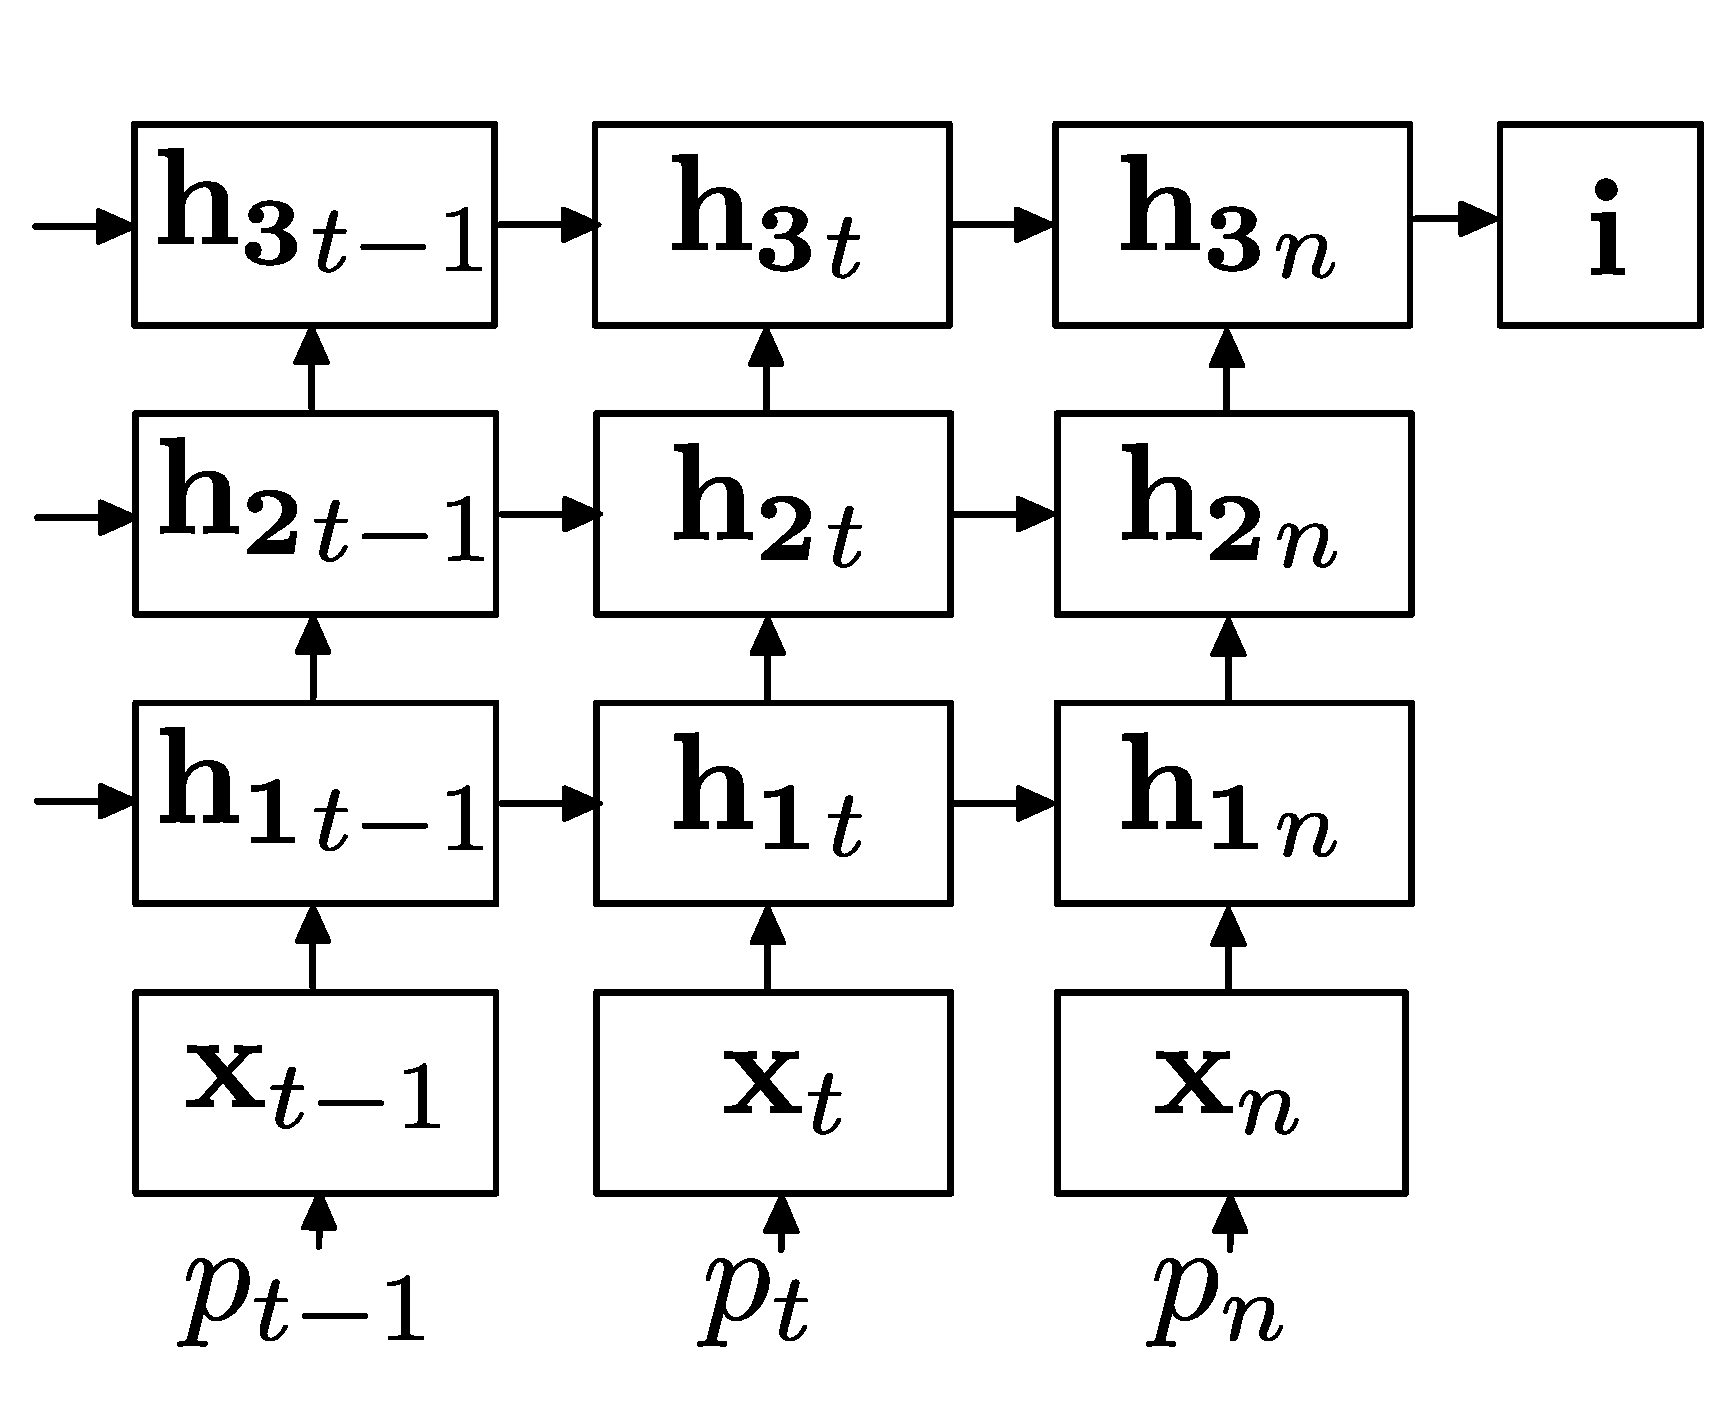
\includegraphics[scale=0.2]{architecture.pdf}
  \caption{A three-timestep slice of the stacked recurrent architecture with three hidden layers.}
  \label{fig:architecture}
\end{figure}

Gated Recurrent Units (GRU) were introduced in
\newcite{cho2014properties} and \newcite{chung2014empirical} as an
attempt to alleviate the problem of vanishing gradient in standard
simple recurrent nets as known since the work of
\newcite{elman1990finding}. GRUs have a linear shortcut through
timesteps which bypasses the nonlinearity and thus promotes gradient
flow.
Specifically, a GRU computes the hidden state at current time step, $\mathbf{h}_{t}$, as the
linear combination of previous activation $\mathbf{h_{t-1}}$, and a new
{\it candidate} activation $\mathbf{\tilde{h}}_t$:
%

\begin{equation}
  \mathrm{gru}(\mathbf{x}_t, \mathbf{h}_{t-1}) = (1 - \mathbf{z}_t)\odot \mathbf{h}_{t-1} + \mathbf{z}_t \odot \mathbf{\tilde{h}}_t
\vspace{-.1cm}
\end{equation}
%
where $\odot$ is elementwise multiplication, and the update gate
activation $\mathbf{z_{t}}$ determines the amount of new information
mixed in the current state:
%

\begin{equation}
\label{eq:gru-update}
   \mathbf{z}_t = \sigma_s(\mathbf{W}_z \mathbf{x}_t + \mathbf{U}_z \mathbf{h}_{t-1})
\end{equation}
%
The candidate activation is computed as:
%
\begin{equation}
\label{eq:gru-cand}
   \mathbf{\tilde{h}}_t = \sigma(\mathbf{W} \mathbf{x}_t + \mathbf{U}(\mathbf{r}_t \odot \mathbf{h}_{t-1}))
\end{equation}
%
The reset gate $\mathbf{r_{t}}$ determines how much of the current
input $\mathbf{x_{t}}$ is mixed in the previous state
$\mathbf{h}_{t-1}$ to form the candidate activation:
%
\begin{equation}
\label{eq:gru-reset}
   \mathbf{r}_t = \sigma_s(\mathbf{W}_r \mathbf{x}_t + \mathbf{U}_r \mathbf{h}_{t-1})
\end{equation}

By applying the $\mathrm{gru}$ function repeatedly a GRU layer maps a
sequence of inputs to a sequence of states:
\begin{equation}
  \mathrm{GRU}(\mathbf{X}, \mathbf{h}_0) = \mathrm{gru}(\mathbf{x}_n, \dots, \mathrm{gru}(\mathbf{x}_2, \mathrm{gru}(\mathbf{x}_1, \mathbf{h}_0)))
\end{equation}
where $\mathbf{X}$ stands for the matrix composed of input column vectors
$\mathbf{x}_1, \ldots, \mathbf{x}_n$. Two or more GRU layers can be composed into a stack: 
\begin{equation}
\mathrm{GRU}_2(\mathrm{GRU}_1(\mathbf{X}, {\mathbf{h_1}}_{0}), {\mathbf{h_2}}_{0}).
\end{equation}
In our version of the Stacked GRU architecture we use {\it residualized} layers:
\begin{equation}
\mathrm{GRU_{res}}(\mathbf{X}, \mathbf{h}_0) = \mathrm{GRU}(\mathbf{X}, \mathbf{h}_0) + \mathbf{X}
\end{equation}
Residual convolutional networks were introduced by
\newcite{he2015deep}, while \newcite{oord2016pixel} showed their
applicability to recurrent architectures. We adopt residualized layers
here are we observed they speed up learning in stacks of several
GRU layers.

Our gated recurrent units use steep sigmoids for gate activations: \[
\sigma_s(z) = \frac{1}{1 + \exp(-3.75z)} 
\]
and rectified linear units clipped between 0 and 5 for the unit
activations:
\[
\sigma(z) = \mathrm{clip(0.5(z+\mathrm{abs}(z)), 0, 5)}
\]

There are two more components of our {\sc Phon GRU} model: the
phoneme encoding layer, and mapping from the final state of the top GRU
layer to the image feature vector.
The phoneme encoding layer is a simply a lookup table $\mathbf{E}$ whose
columns correspond to one-hot-encoded phoneme vectors. The input
phoneme $p_t$ of utterance $p$ at each step $t$ indexes into the
encoding matrix and produces the input column vector:
\begin{equation}
  \mathbf{x}_t = \mathbf{E}[:,p_t].
\end{equation}
Finally, we map the final state of the top GRU layer ${\mathbf{h_K}}_n$
to the vector of image features using a fully connected layer:

\begin{equation}
  \hat{\mathbf{i}} = \mathbf{I} {\mathbf{h_K}}_n
\end{equation}

Our main interest lies in  recurrent phoneme-level modeling. However in order to
put the performance of the phoneme-level {\sc Phon GRU} into
perspective we compare it to the following two other models.


\subsection{Word GRU}
The architecture of this model is the same as {\sc Phon GRU} with
the difference that we use words instead of phonemes as input symbols,
use learnable word embeddings instead of fixed one-hot phoneme
encodings, and reduce the number of layers in the GRU stack. See
\ref{sec:experiments} for details.
\subsection{Word Sum}
The second model we use for comparison is word-based non-sequential
model, consisting of a word embedding matrix, a vector sum operator,
and a mapping to the image vector feature vector:
\begin{equation}
  \label{eq:sum}
  \hat{\mathbf{i}} = \mathbf{I} \sum_{t=1}^n \mathbf{E}[:,w_t]
\end{equation}
where $w_t$ is the word at position $t$ in the input utterance.
This model simply learns word embeddings which are then summed into a
single vector and projected to the target image vector. Thus this model does
not have access to word sequence information, and is a distributed
analog of a bag-of-words model.
